\documentclass[../main]{subfiles}

\begin{document}

\clearpage

\setcounter{eqnarray}{0}
\setcounter{equation}{0}
\setcounter{figure}{0}

\part*{第11回}

\section{電磁誘導}

{\bf 復習} \\
静電場では
\begin{eqnarray*}
{\rm div}{\bf E}=\frac{\rho}{\varepsilon_0},{\rm rot}{\bf E}={\bf 0} \\
{\rm div}{\bf B}=0,{\rm rot}{\bf B}=\mu_0{\bf i}
\end{eqnarray*}
電荷は保存され
\begin{eqnarray*}
\frac{\partial \rho}{\partial t}+{\rm div}{\bf i}=0
\end{eqnarray*}
電荷に働くLorentz力は
\begin{eqnarray*}
{\bf F}=q({\bf E}+{\bf v} \times {\bf B})
\end{eqnarray*}
電場が時間変化するときは${\rm rot}{\bf E}={\bf 0},{\rm rot}{\bf B}=\mu_0{\bf i}$の右辺に補正項が要る.

\subsection{Faradayの電磁誘導の法則}

\begin{itembox}[c]{有向ループCを貫く磁束}
有向ループCを貫く磁束は,Cをふちとする曲面Sにわたる面積分であり,
\begin{eqnarray}
\Phi = \int_{S} {\bf B} \cdot {\bf dS}
\end{eqnarray}
表裏の定め方はAmp\`ereの法則のときと同様.
\end{itembox}
注:Sの取り方によらない.
\begin{eqnarray*}
\int_{S}{\bf B}\cdot{\bf dS} -\int_{S'}{\bf B}\cdot{\bf dS} = \int_{S \cup \overline{S}} {\bf B}\cdot{\bf dS} = \int {\rm div}{\bf B} dV = 0
\end{eqnarray*}
$\Phi$の単位は ${\rm Wb = JA^{-1}}$
\begin{eqnarray*}
\Phi = \int {\bf B} (x,y,z,t) \cdot {\bf dS} = \Phi (t)
\end{eqnarray*}
\\
\begin{itembox}[c]{Cに沿う起電力}
\begin{eqnarray}
\mathcal{E} = \int_{C} {\bf E} \cdot {\bf dl} [JC^{-1}]
\end{eqnarray}
\end{itembox}
注:静電場だとStokesの定理より
\begin{eqnarray*}
\mathcal{E} = \int_{C} {\bf E} \cdot {\bf dl} = \int_{S} {\rm rot}{\bf E} \cdot {\bf dS} = 0
\end{eqnarray*}

\begin{itembox}[c]{Faradayの法則}
磁束$\Phi$が時間とともに変化するとそれを妨げる(打ち消す)向きに,Cに起電力$\mathcal{E}$が生じる.この起電力を誘導起電力という.(Cが導線であれば,電流が生じる.)誘導起電力の大きさは
\begin{eqnarray}
\mathcal{E}=-\frac{d \Phi}{dt}
\end{eqnarray}
単位は${\rm Wbs^{-1}=JA^{-1}s^{-1}=JC^{-1}}$ \\
起電力の向きに関する法則はLenzの法則ともいう.
\end{itembox}
{\bf 例}:Cは一定,{\bf B}が時間変化する場合. \\

\begin{figure}[htbp]
 \begin{center}
  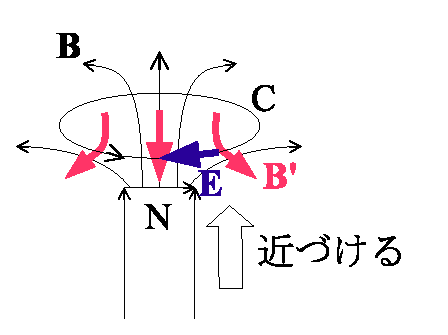
\includegraphics[width=80mm]{11.1.eps}
 \end{center}
 \caption{}
 \label{fig:one}
\end{figure}

\begin{eqnarray*}
\frac{d \Phi}{dt} > 0,\mathcal{E}<0
\end{eqnarray*}
Cにおける{\bf E}はCの向きと逆.{\bf B}'は{\bf B}を打ち消す向き. \\
\\
{\bf 例}:{\bf B}が一定,Cが時間変化する場合. \\

\begin{figure}[htbp]
 \begin{center}
  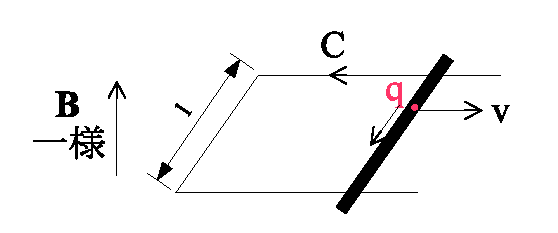
\includegraphics[width=80mm]{11.2.eps}
 \end{center}
 \caption{}
 \label{fig:one}
\end{figure}

\begin{eqnarray*}
\Phi = - Bl(vt+const.) \\
\mbox{Lorentz力} \quad F = qvB \\
\end{eqnarray*}
のとき
\begin{eqnarray*}
\mathcal{E} = \int_{C} {\bf E} \cdot {\bf l} = - vBl = -\frac{d \Phi}{dt}
\end{eqnarray*}
となり,Lorentz力と整合する.
\\
さて,Faradayの法則(3)を出発点として,静電場で成り立つ${\rm rot}{\bf E}=0$を補正する. \\
左辺の起電力を有向ループCに沿う線積分に書き換えると,式(2)より,
\begin{eqnarray*}
\int_{C} {\bf E} \cdot {\bf dl} = -\frac{d \Phi}{dt}
\end{eqnarray*}
右辺の磁束を磁束密度の,有向ループCをふちとする曲面Sにわたる面積分で書き換えると,式(1)より,
\begin{eqnarray*}
\int_{C} {\bf E} \cdot {\bf dl} = -\frac{d}{dt} \int_{S} {\bf B} \cdot {\bf dS}
\end{eqnarray*}
Stokesの定理によって,左辺の線積分を面積分に書き換えると,
\begin{eqnarray*}
\int_{S} {\rm rot}{\bf E} \cdot {\bf dS} = -\frac{d}{dt} \int_{S} {\bf B} \cdot {\bf dS}
\end{eqnarray*}
右辺の時間微分を磁束密度にかけると,
\begin{eqnarray*}
\int_{S} {\rm rot}{\bf E} \cdot {\bf dS} = -\int_{S} \frac{\partial {\bf B} }{\partial t} \cdot {\bf dS}
\end{eqnarray*}
曲面Sは任意であるから,

\begin{itembox}[c]{電場の回転}
\begin{eqnarray*}
{\rm rot}{\bf E} = -\frac{\partial {\bf B} }{\partial t}
\end{eqnarray*}
\end{itembox}


\subsection{自己誘導,相互誘導}
\begin{eqnarray*}
\Phi = \int_{S} {\bf B} \cdot {\bf dS} = LI
\end{eqnarray*}
比例定数Lを自己誘導係数(インダクタンス)といい,単位は${\rm WbA^{-1}=H}$ \\
{\bf 例}:ソレノイド \\
単位長の巻き数n,長さl,断面積Sのソレノイドを考える.
\begin{eqnarray*}
B = \mu_0 n I \\
\Phi = BSln = \mu_0 n^2 l S I 
\end{eqnarray*}
よってソレノイドの自己インダクタンスは,
\begin{eqnarray*}
L=\mu_0 n^2 l S
\end{eqnarray*}
\\

\begin{figure}[htbp]
 \begin{center}
  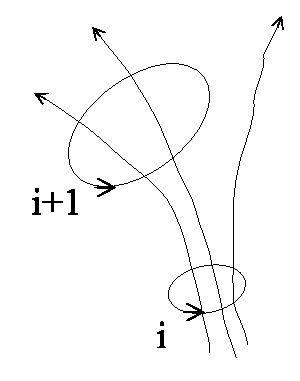
\includegraphics[width=50mm]{11.3.eps}
 \end{center}
 \caption{}
 \label{fig:one}
\end{figure}

一般に,i番目のループを貫く磁束を$\Phi_i {\rm (I_1,I_2...I_n) (i=1,2...n)}$とすると,

\begin{itembox}[c]{i番目のループを貫く磁束}

\begin{eqnarray*}
\Phi_i(I_1,...,I_n) = \sum_{j=i}^{n}L_{ij}I_j \\
L_{ii}:\mbox{自己インダクタンス} \\
L_{ij}(i \neq j) : \mbox{相互インダクタンス}
\end{eqnarray*}

\end{itembox}



\newpage

{\bf 例}:単位あたりの巻き数$n_1,n_2$,断面積$S_1,S_2$のソレノイド \\


\begin{figure}[htbp]
 \begin{center}
  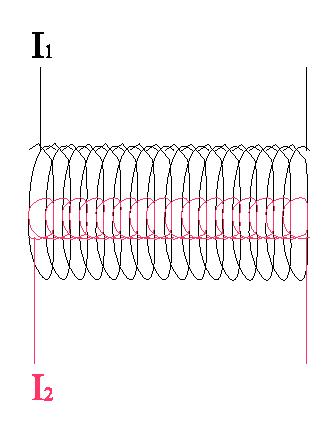
\includegraphics[width=50mm]{11.4.eps}
 \end{center}
 \caption{}
 \label{fig:one}
\end{figure}

\begin{eqnarray*}
\Phi_1(I_1=0,I_2) = L_{11}0+L_{12}I_2 \\
\Phi_2(I_1,I_2=0) = L_{21}I_1+L_{22}0
\end{eqnarray*}
また,
\begin{eqnarray*}
\Phi_1(I_1=0,I_2) = \mu_0 n_2 I_2 \cdot l n_1 S_2 \\
\Phi_2(I_1,I_2=0) = \mu_0 n_1 I_1 \cdot l n_2 S_2
\end{eqnarray*}
よって
\begin{eqnarray*}
L_{12}=L_{21}=\mu_0n_1n_2lS_2
\end{eqnarray*}
一般に$L_{ij}=L_{ji}$が成り立つ. \\
\\
{\bf 交流回路} \\

\begin{figure}[htbp]
 \begin{center}
  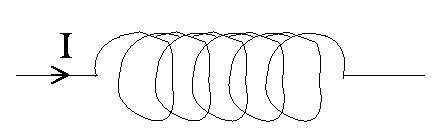
\includegraphics[width=50mm]{11.5.eps}
 \end{center}
 \caption{}
 \label{fig:one}
\end{figure}

コイルの起電力の大きさは
\begin{eqnarray*}
\left| \frac{d \Phi}{dt} \right| = L\left|\frac{d I}{dt} \right|
\end{eqnarray*}
\\

\begin{figure}[htbp]
 \begin{center}
  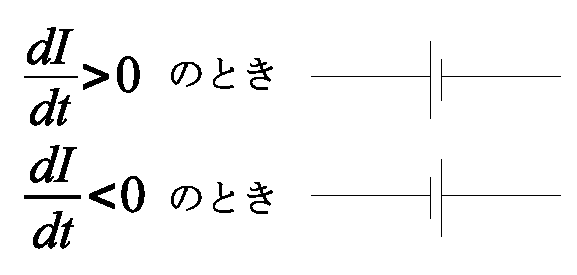
\includegraphics[width=50mm]{11.6.eps}
 \end{center}
 \caption{}
 \label{fig:one}
\end{figure}

\newpage

{\bf LCR回路} \\

\begin{figure}[htbp]
 \begin{center}
  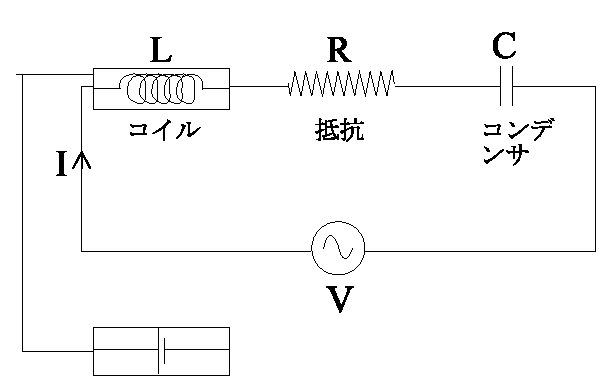
\includegraphics[width=80mm]{11.7.eps}
 \end{center}
 \caption{}
 \label{fig:one}
\end{figure}

\begin{eqnarray*}
L\frac{dI}{dt}+RI + \frac{1}{C}Q = V
\end{eqnarray*}
両辺を時間微分して,$\frac{dQ}{dt}=I$と書き換えると,
\begin{eqnarray*}
L\frac{d^2 I}{dt^2}+R\frac{dI}{dt}+\frac{I}{C} = \frac{dV}{dt}
\end{eqnarray*}
となり,Iについての2階の微分方程式が得られる. \\
とくに$\frac{dV}{dt}=0$でも電流は振動する. \\
抵抗が0であるときはLC回路といい(ただし$\frac{dV}{dt}=const.$),電流Iは単振動する.

\end{document}




